% !TEX root = replicas_draft.tex


\section{Comments on reconstructing the interior}
\label{sec:Dictionary}

The island contribution to the entropy of a flat space region $R$ indicates there is a dictionary between the island $I$ and $R$ in the sense of entanglement wedge reconstruction in AdS/CFT. We could discuss this in general but for concreteness consider the two interval case discussed in the previous section. Let's take the state at late times such that the entropy of $R$ has plateaued and its entropy receives a contribution from the island as shown in figure \ref{JLMSlatetime}.

The first step to establishing a dictionary is to define a subspace of states which have the same ``entanglement wedge'' or island. This defines what we will call the code subspace  ${\cal H}_{code}$, which we imagine can be prepared via the Euclidean path integral with possible operator insertions. By having the same island we mean that the leading saddle points in the Renyi computations are only modified perturbatively. This naturally puts restrictions on the size of the allowed code subspace for which the statements of this section hold, see for example \cite{Hayden:2018khn, hayden2017approximate}. 


We assume that the full Hilbert space of our model is that of the two flat space regions including their boundary, which we write as $ {\cal H}_{\rm Left} \otimes {\cal H}_{\rm Right}$. The region $R$ that we are considering is a tensor factor of this Hilbert space, where we can write
\begin{align}
 {\cal H}_{\rm Left} \otimes {\cal H}_{\rm Right} = {\cal H}_R \otimes {\cal H}_{\bar R}
\end{align}
where $\bar{R}$ is the complement of the region $R$ in the flat space region including the boundary points. 

The code subspace ${\cal H}_{code}$ is a subspace of $ {\cal H}_{\rm Left} \otimes {\cal H}_{\rm Right}$. However, the code subspace also has a simpler description in terms of the combined description of gravity plus the flat space region as that of effective field theory on a Cauchy slice of the full spacetime. This is the description where the state is prepared using the semi-classical saddle via the Euclidean black hole solution. 
The code subspace should be thought of as isomorphic to this. Therefore, the code subspace admits the decomposition\footnote{This should be understood as approximate up to usual issues of the non-factorizability of continuum QFT.}
\begin{align}
{\cal H}_{code} \cong {\cal H}_{R} \otimes {\cal H}_{D} \otimes {\cal H}_{I} 
\end{align}
where the region $D$ is the complement of $R \cup I$ on the Cauchy slice. The decomposition is shown in figure \ref{JLMSlatetime}. It is within this effective description that for any state in the code subspace $|i \rangle \in {\cal H}_{code}$, we have
\begin{align}
S({\bold \rho}_{R}^{i}) = S(\tilde{\rho}_{RI}^{i}) + {\mathrm{Area}[\partial I] \over 4 G_N}
\end{align}
where $\rho^i_{R}$ is what you get by tracing out $\bar{R}$ in the full quantum description ${\cal H}_{\rm Left} \otimes {\cal H}_{\rm Right}$, and $\tilde{\rho}_{RI}^i$ is the density matrix obtained by tracing out the complement of $RI$ in the semi-classical description consisting of quantum fields on a classical geometry.

\begin{figure}
\begin{center}
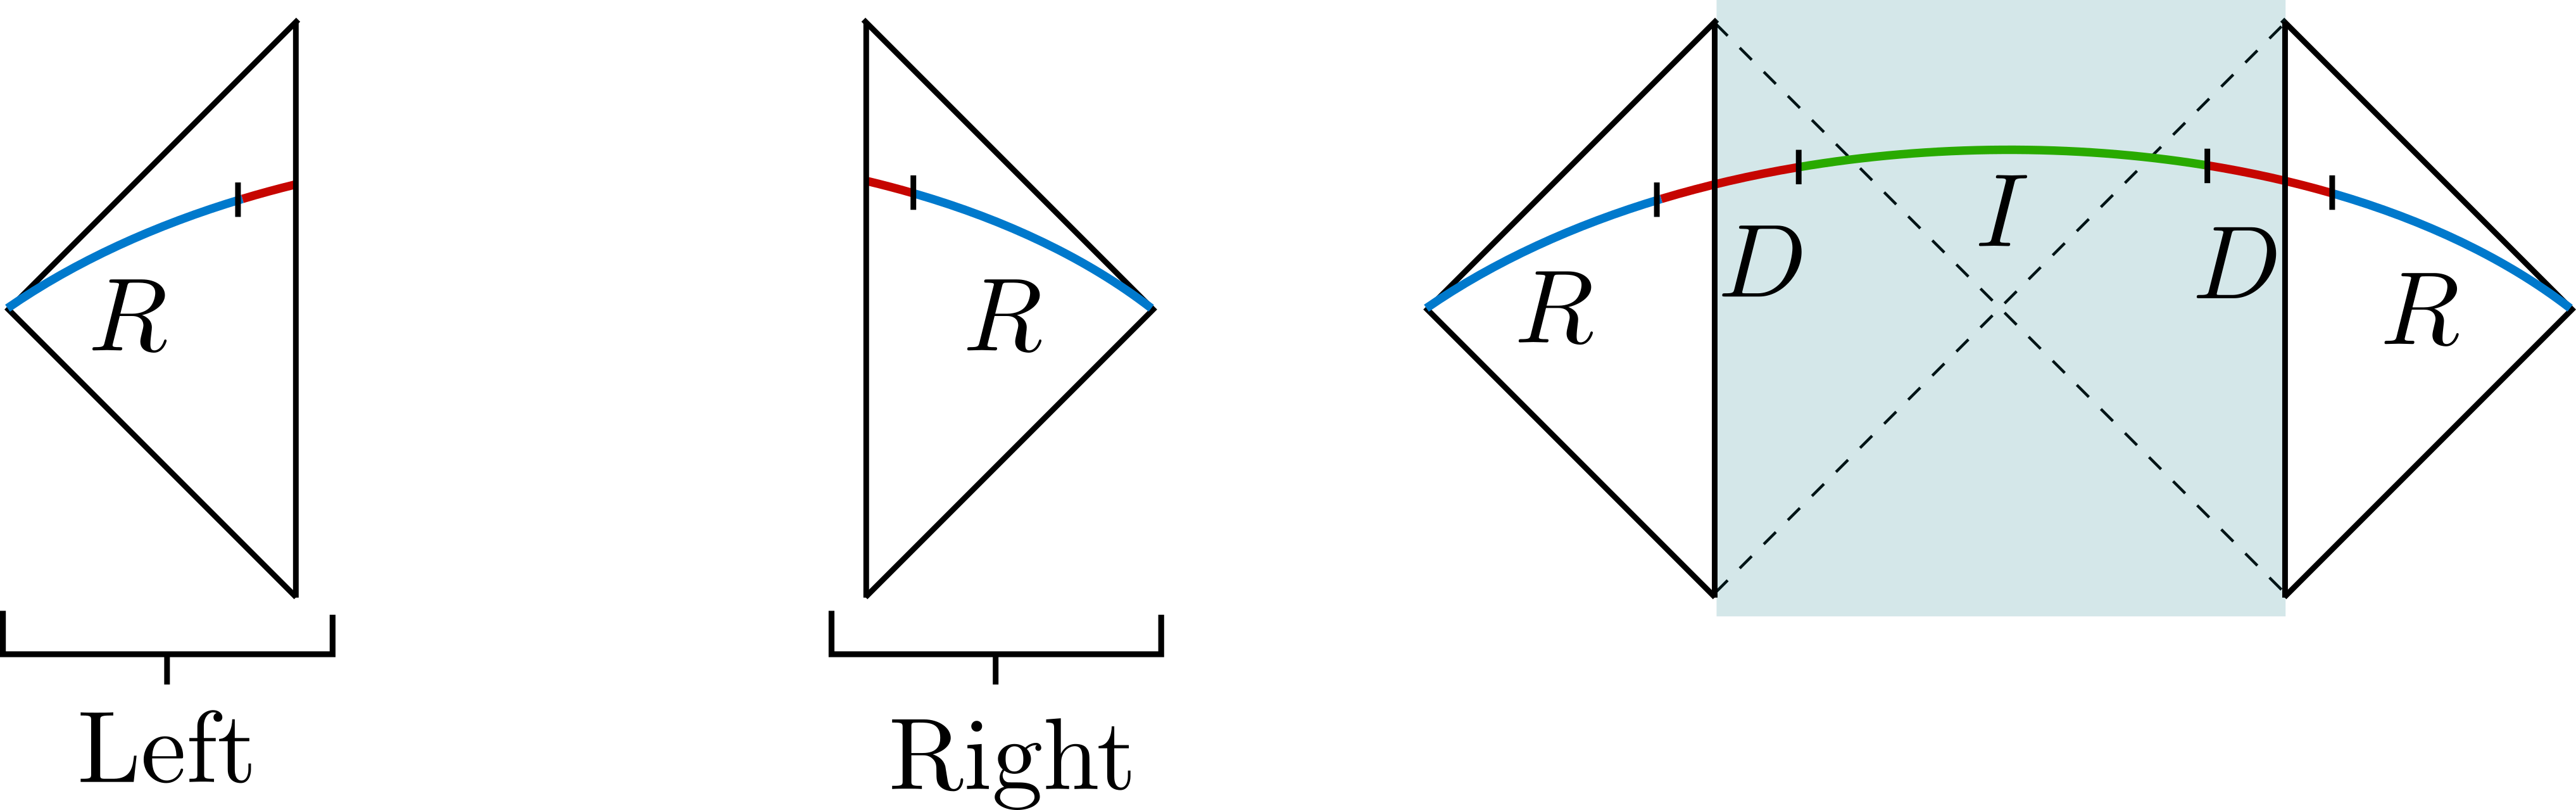
\includegraphics[scale=0.6]{figures/JLMSlatetime.jpg}
(a) ~~~~~~~~~~~~~~~~~~~~~~~~~~~~~~~~~~~~~~~~~~~~~~~~~~~~~~~ ~~~~~(b)
\end{center}
\caption{\small (a) The full Hilbert space is the product Hilbert space of the entire left and right flat space regions including the boundary points. The region $R$ we are interested in is a union of two subregions in the two flat space regions. (b) The effective state used in the island prescription is the semi-classical state defined on the Cauchy slice of the full system. $R$ is the same region in the flat space region whose exact entropy we are computing, $I$ is the island, and $D$ is the complement of the two.
\label{JLMSlatetime}}
\end{figure}

The validity of the island formula (for a fixed island) within the code subspace implies the equivalence of the relative entropy in the exact state and the semi-classical state:
\begin{align} \la{RelEnt}
S_\mathrm{Rel}(\rho_{R} | \sigma_{R}) = S_\mathrm{Rel}(\tilde{\rho}_{ R I} | \tilde{\sigma}_{ R I})
\end{align}
A similar observation in the context of AdS/CFT \cite{Jafferis:2015del} was key in proving entanglement wedge reconstruction \cite{Dong:2016eik} using the quantum error correction interpretation of the duality\cite{Almheiri:2014lwa}. The same line of argument can be applied here to establish the dictionary. In particular, one can show that for any operator ${\cal O}_I$ (and its Hermitian conjugate) acting within the ${\cal H}_{code}$ and supported on the island one can find an operator supported on $R$ such that:
\begin{align}
{\cal O}_I | i \rangle  &= {\cal O}_{R} | i \rangle \\
{\cal O}_I^\dagger | i \rangle  &= {\cal O}_{R}^\dagger | i \rangle
\end{align}
The operator $ {\cal O}_{R}$ is given by a complicated operator on ${R}$ involving the matrix elements of ${\cal O}_I$ within the code subspace. 



In summary, we are using the fine grained entropy formula to understand how the interior is encoded in the full Hilbert space. The relative entropy equality \eqref{RelEnt} tells us that distinguishable states in the interior (the island) are also distinguishable in the radiation, within the full exact quantum description. 













 
 
 
